\section{Umwelt}\label{sec:solutions}

Im folgenden Kapitel wird der Abbau und die Nutzung von
Tantal und die daraus resultierenden Folgen für die Umwelt untersucht.
Das Hauptaugenmerk liegt dabei auf der Bewertung einzelner Indikatoren im Bezug
auf deren Beitrag zur Nachhaltigkeit.
\subsection{Indikatoren}

\paragraph{Rohstoffverbrauch / Rohstoffbestand}
Dieser Indikator befasst sich mit dem weltweiten Verbrauch des Rohstoffs
Tantal und den Auswirkungen auf dessen globalen Bestand. Ein steigender
Verbrauch beziehungsweise ein sinkender Bestand wird im Bezug auf die
Nachhaltigkeit als negativ eingestuft.

\paragraph{Abbau / Regelung}
Um eine Aussage über die Nachhaltigkeit der Tantalgewinnung machen zu können,
muss der direkte Einfluss des Abbaus auf die Umwelt betrachtet werden. Dabei
soll untersucht werden, welche Methoden dafür angewandt werden und ob diese
risikobehaftet sind, zum Beispiel aufgrund von toxischen Emissionen.

\paragraph{Naturraum / Landschaft}
Massgebend für die Bewertung dieses Indikators ist der Einfluss der
Tantalgewinnung auf den Naturraum im betroffenen Abbaugebiet und die mittel- bis
langfristige Veränderung der Landschaft.

\subsection{Bewertung}
Die globale Fördermenge von Tantal lag \textbf{2013} bei geschätzten 1300 Tonnen. Davon wurden
knapp 40\% für die Herstellung von Kondensatoren verwendet. Prognosen gehen
davon aus, dass sich dieser Bedarf bis ins Jahr \textbf{2035} mehr als
verdoppeln wird ~\cite{Weltweit69:online}.
Zum  weltweiten Bestand lassen sich nur schwer Aussagen machen, da sich ein grosser
Teil des Vorkommens in Konfliktregionen befindet und somit kein kontrollierter
Abbau stattfindet. Das U.S Geological Survey (USGS) geht jedoch davon aus, dass
im Jahr 2018 noch über 110'000 Tonnen an Reserven vorhanden
sind ~\cite{ober2018mineral}.
In Anbetracht des prognostizierten Verbrauches werden ohne Gegenmassnahmen
mittelfristig Engpässe auftreten. Schätzungen darüber, wann dies sein wird,
reichen dabei von 15 bis 125 Jahren ~\cite{behrendt2007seltene}. Durch die Einführung neuer Technologien und dem
damit einhergehenden kompletten Verzicht auf Tantal in der ICT bis zum Jahr \textbf{2035} kann dies
zwar aufgeschoben, jedoch nicht verhindert werden. Dies liegt einerseits daran,
dass auch in anderen Anwendungsgebieten von Tantal mit einem enormen Anstieg des
Verbrauches gerechnet wird. Andererseits werden heute nur ungefähr 10 - 20\%
aller aus Tantal gefertigten Bauteile am Ende ihrer Nutzung recyclet ~\cite{behrendt2007seltene}.

\begin{figure}[h]
\centering
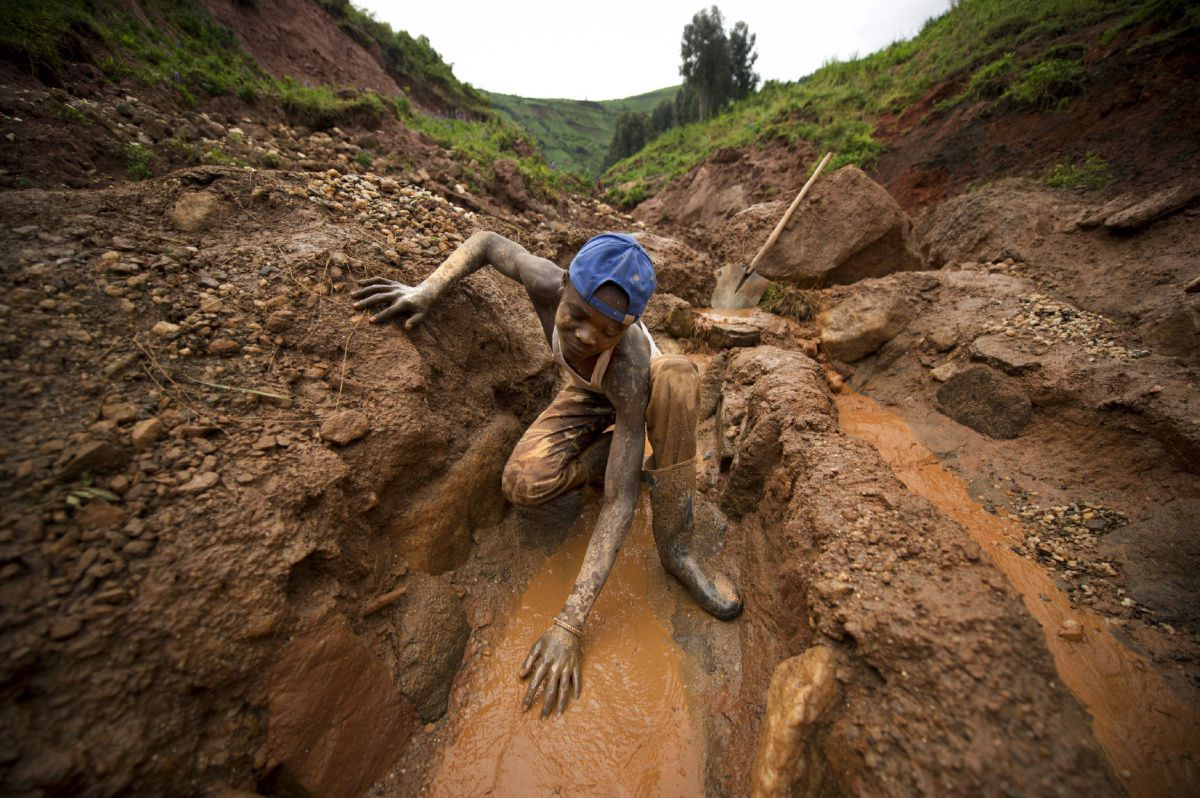
\includegraphics[width=0.8\textwidth]{coltan_in_thecongo1}
\caption{Arbeiter in einer Coltan Mine im Kongo ~\cite{Coltanam17:online}}
\label{}
\end{figure}

Da Tantal in der Natur nicht in reiner Form sondern als Bestandteil verschiedener
Mineralien vorkommt, wobei Coltan (\textbf{Col}umbit-\textbf{Tan}talit) das am
weitesten verbreitete ist, betrachten wir in der Folge den \textbf{Abbau} von Coltan.
Da Coltan in den oberen Gesteinsschichten vorkommt, sind die meisten
Coltan-Minen oberflächlich und die Gewinnung nicht sehr
aufwendig ~\cite{reetsch2008effects}. Ausserdem werden dabei keine toxischen
Stoffe verwendet wie bei anderen Mineralien. Die Tatsache, dass die Förderung
mit einfachen Mitteln möglich ist, führt jedoch auch dazu, dass in den
Konfliktregionen Afrikas viele unkontrollierte Minen entstehen. In diesen meist
unter der Kontrolle von lokalen Milizen betriebenen Minen finden Vorschriften
bezüglich des Umweltschutzes in der Regel keine Beachtung ~\cite{bleischwitz2012coltan}.
Untersuchungen belegen, dass zwar erhöhte Werte von toxischen Stoffen wie Arsen
und Uran im Boden und den Gewässern im Umkreis der Minen messbar sind, diese
jedoch unter den von der WHO festgelegten Grenzwerten ~\cite{environmental_management} liegen.

Ganz im Gegensatz zu den direkten Folgen des Coltan-Abbaus, welche nicht extrem
ins Gewicht fallen bezüglich der Nachhaltigkeit, ziehen die Folgen für den
\textbf{Naturraum} der betroffenen Regionen gravierende Konsequenzen mit sich.
So werden grosse Flächen Wald gerodet um die Minen zu errichten. Dies führt
dazu, dass die Böden unfruchtbar und anfällig auf Bodenerosionen
werden ~\cite{environmental_management}.

\begin{figure}[h]
\centering
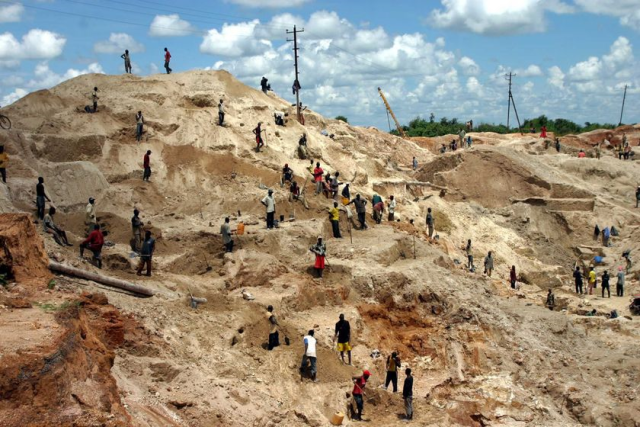
\includegraphics[width=0.8\textwidth]{erosion}
\caption{Bodenerosion verursacht durch Minen ~\cite{Coltanmi34:online}}
\label{}
\end{figure}
\pagebreak

Andererseits liegen viele der Minen der Demokratischen Republik Kongo in
Naturschutzreservaten. Durch die Zerstörung ihres Lebensraumes und die gezielte
Jagd auf die Tiere durch Minenarbeiter verringern sich die Bestände der bereits
vom Aussterben bedrohten Tierarten, wie zum Beispiel dem Berggorilla, dramatisch.
Sollte die Nachfrage nach Tantal tatsächlich so ansteigen wie prognostiziert,
könnte es \textbf{2035} bereits zu spät sein für einige dieser Arten.
Durch den Verzicht auf Tantal durch die ICT-Industrie könnte hier ein wertvoller
Beitrag geleistet werden zur Erhaltung der Artenvielfalt.

\begin{table}[h]
  \centering
  \begin{tabular}{l|ccc}                                    & \textbf{2013} & \textbf{2035} & \textbf{2035 mit Annahme}
    \\ \hline Rohstoffverbrauch / Rohstoffbestand                 & 5             & 2             & 4 
    \\ Abbau / Regelung                                           & 7             & 5             & 6
    \\ Natrurraum / Landschaft                                    & 3             & 2             & 3
    \\ \hline \textbf{Endbewertung}                               & 5             & 3             & 4\(\frac{1}{3}\)
  \end{tabular}
  \caption{Resultat ökologische Analyse}
\end{table}
